\begin{quote}\small\textbf{观课提示}\quad 先预测不同学习率下是靠近、振荡还是发散，再运行同一个二次损失实验。

\href{https://www.youtube.com/watch?v=IHZwWFHWa-w}{原课程视频}\quad\href{https://vitael04213.github.io/3blue1brown-notes/lessons/gradient-descent.html}{本节网页与媒体}\quad\href{https://vitael04213.github.io/3blue1brown-notes/lab.html\#gradient}{参数实验}
\end{quote}
\begin{figure}[htbp]\centering
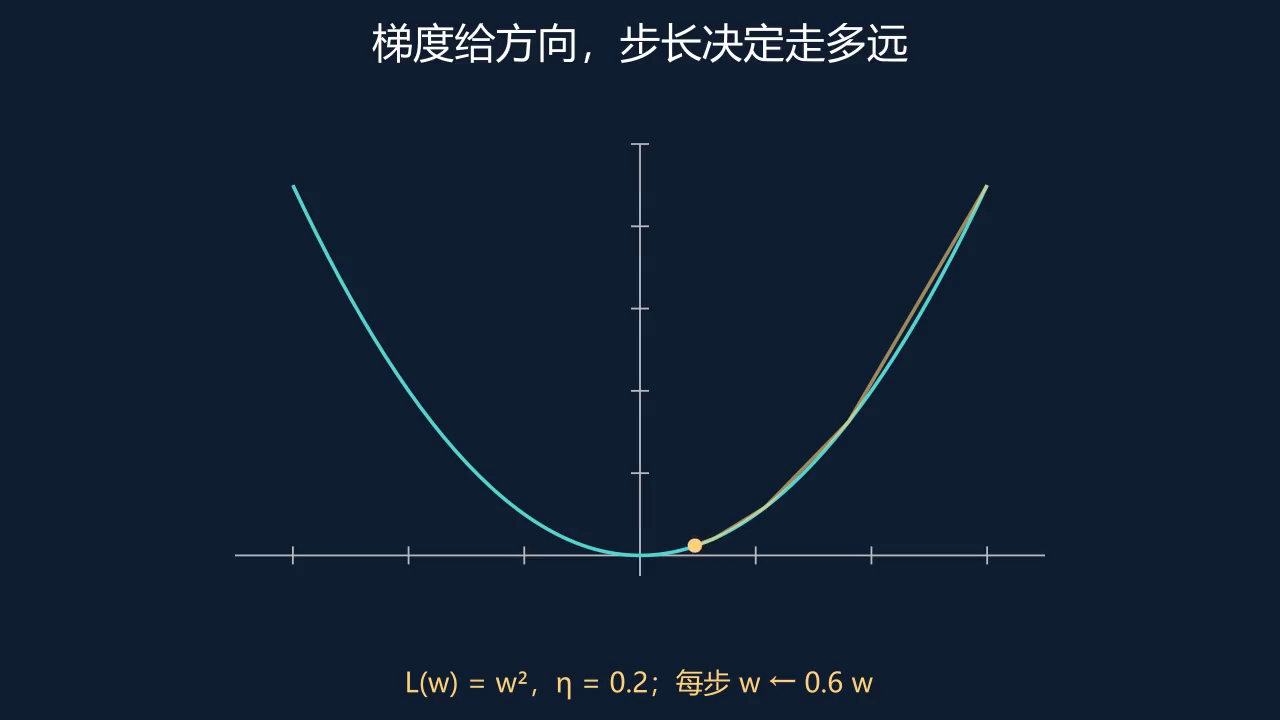
\includegraphics[width=0.98\linewidth]{figures/GradientDescent.png}
\caption{二次损失上的更新轨迹；这里学习率为 0.2。网页可改用过大步长观察发散。本项目原创 Manim 动画关键帧；完整动画与操作入口见本节网页。}
\end{figure}
